\documentclass[twoside]{book}

% Packages required by doxygen
\usepackage{fixltx2e}
\usepackage{calc}
\usepackage{doxygen}
\usepackage[export]{adjustbox} % also loads graphicx
\usepackage{graphicx}
\usepackage[utf8]{inputenc}
\usepackage{makeidx}
\usepackage{multicol}
\usepackage{multirow}
\PassOptionsToPackage{warn}{textcomp}
\usepackage{textcomp}
\usepackage[nointegrals]{wasysym}
\usepackage[table]{xcolor}

% Font selection
\usepackage[T1]{fontenc}
\usepackage[scaled=.90]{helvet}
\usepackage{courier}
\usepackage{amssymb}
\usepackage{sectsty}
\renewcommand{\familydefault}{\sfdefault}
\allsectionsfont{%
  \fontseries{bc}\selectfont%
  \color{darkgray}%
}
\renewcommand{\DoxyLabelFont}{%
  \fontseries{bc}\selectfont%
  \color{darkgray}%
}
\newcommand{\+}{\discretionary{\mbox{\scriptsize$\hookleftarrow$}}{}{}}

% Page & text layout
\usepackage{geometry}
\geometry{%
  a4paper,%
  top=2.5cm,%
  bottom=2.5cm,%
  left=2.5cm,%
  right=2.5cm%
}
\tolerance=750
\hfuzz=15pt
\hbadness=750
\setlength{\emergencystretch}{15pt}
\setlength{\parindent}{0cm}
\setlength{\parskip}{3ex plus 2ex minus 2ex}
\makeatletter
\renewcommand{\paragraph}{%
  \@startsection{paragraph}{4}{0ex}{-1.0ex}{1.0ex}{%
    \normalfont\normalsize\bfseries\SS@parafont%
  }%
}
\renewcommand{\subparagraph}{%
  \@startsection{subparagraph}{5}{0ex}{-1.0ex}{1.0ex}{%
    \normalfont\normalsize\bfseries\SS@subparafont%
  }%
}
\makeatother

% Headers & footers
\usepackage{fancyhdr}
\pagestyle{fancyplain}
\fancyhead[LE]{\fancyplain{}{\bfseries\thepage}}
\fancyhead[CE]{\fancyplain{}{}}
\fancyhead[RE]{\fancyplain{}{\bfseries\leftmark}}
\fancyhead[LO]{\fancyplain{}{\bfseries\rightmark}}
\fancyhead[CO]{\fancyplain{}{}}
\fancyhead[RO]{\fancyplain{}{\bfseries\thepage}}
\fancyfoot[LE]{\fancyplain{}{}}
\fancyfoot[CE]{\fancyplain{}{}}
\fancyfoot[RE]{\fancyplain{}{\bfseries\scriptsize Generated by Doxygen }}
\fancyfoot[LO]{\fancyplain{}{\bfseries\scriptsize Generated by Doxygen }}
\fancyfoot[CO]{\fancyplain{}{}}
\fancyfoot[RO]{\fancyplain{}{}}
\renewcommand{\footrulewidth}{0.4pt}
\renewcommand{\chaptermark}[1]{%
  \markboth{#1}{}%
}
\renewcommand{\sectionmark}[1]{%
  \markright{\thesection\ #1}%
}

% Indices & bibliography
\usepackage{natbib}
\usepackage[titles]{tocloft}
\setcounter{tocdepth}{3}
\setcounter{secnumdepth}{5}
\makeindex

% Hyperlinks (required, but should be loaded last)
\usepackage{ifpdf}
\ifpdf
  \usepackage[pdftex,pagebackref=true]{hyperref}
\else
  \usepackage[ps2pdf,pagebackref=true]{hyperref}
\fi
\hypersetup{%
  colorlinks=true,%
  linkcolor=blue,%
  citecolor=blue,%
  unicode%
}

% Custom commands
\newcommand{\clearemptydoublepage}{%
  \newpage{\pagestyle{empty}\cleardoublepage}%
}

\usepackage{caption}
\captionsetup{labelsep=space,justification=centering,font={bf},singlelinecheck=off,skip=4pt,position=top}

%===== C O N T E N T S =====

\begin{document}

% Titlepage & ToC
\hypersetup{pageanchor=false,
             bookmarksnumbered=true,
             pdfencoding=unicode
            }
\pagenumbering{roman}
\begin{titlepage}
\vspace*{7cm}
\begin{center}%
{\Large electrotestgtk \\[1ex]\large 0.\+99 }\\
\vspace*{1cm}
{\large Generated by Doxygen 1.8.11}\\
\end{center}
\end{titlepage}
\clearemptydoublepage
\tableofcontents
\clearemptydoublepage
\pagenumbering{arabic}
\hypersetup{pageanchor=true}

%--- Begin generated contents ---
\chapter{Data Structure Index}
\section{Data Structures}
Here are the data structures with brief descriptions\+:\begin{DoxyCompactList}
\item\contentsline{section}{\hyperlink{structgui__comp}{gui\+\_\+comp} \\*Struct with pointers to all gui and data parts }{\pageref{structgui__comp}}{}
\end{DoxyCompactList}

\chapter{File Index}
\section{File List}
Here is a list of all files with brief descriptions\+:\begin{DoxyCompactList}
\item\contentsline{section}{\hyperlink{calc__result__box_8c}{calc\+\_\+result\+\_\+box.\+c} }{\pageref{calc__result__box_8c}}{}
\item\contentsline{section}{\hyperlink{calc__result__box_8h}{calc\+\_\+result\+\_\+box.\+h} }{\pageref{calc__result__box_8h}}{}
\item\contentsline{section}{\hyperlink{coupling__box_8c}{coupling\+\_\+box.\+c} }{\pageref{coupling__box_8c}}{}
\item\contentsline{section}{\hyperlink{coupling__box_8h}{coupling\+\_\+box.\+h} }{\pageref{coupling__box_8h}}{}
\item\contentsline{section}{\hyperlink{electrotestgtk_8c}{electrotestgtk.\+c} }{\pageref{electrotestgtk_8c}}{}
\item\contentsline{section}{\hyperlink{electrotestgtk_8h}{electrotestgtk.\+h} }{\pageref{electrotestgtk_8h}}{}
\item\contentsline{section}{\hyperlink{helper__functions_8c}{helper\+\_\+functions.\+c} }{\pageref{helper__functions_8c}}{}
\item\contentsline{section}{\hyperlink{helper__functions_8h}{helper\+\_\+functions.\+h} }{\pageref{helper__functions_8h}}{}
\item\contentsline{section}{\hyperlink{libcomponent_8h}{libcomponent.\+h} }{\pageref{libcomponent_8h}}{}
\item\contentsline{section}{\hyperlink{libpower_8h}{libpower.\+h} }{\pageref{libpower_8h}}{}
\item\contentsline{section}{\hyperlink{libresistance_8h}{libresistance.\+h} }{\pageref{libresistance_8h}}{}
\item\contentsline{section}{\hyperlink{resistor__box_8c}{resistor\+\_\+box.\+c} }{\pageref{resistor__box_8c}}{}
\item\contentsline{section}{\hyperlink{resistor__box_8h}{resistor\+\_\+box.\+h} }{\pageref{resistor__box_8h}}{}
\item\contentsline{section}{\hyperlink{voltage__box_8c}{voltage\+\_\+box.\+c} }{\pageref{voltage__box_8c}}{}
\item\contentsline{section}{\hyperlink{voltage__box_8h}{voltage\+\_\+box.\+h} }{\pageref{voltage__box_8h}}{}
\end{DoxyCompactList}

\chapter{Data Structure Documentation}
\hypertarget{structgui__comp}{}\section{gui\+\_\+comp Struct Reference}
\label{structgui__comp}\index{gui\+\_\+comp@{gui\+\_\+comp}}


Struct with pointers to all gui and data parts.  




{\ttfamily \#include $<$electrotestgtk.\+h$>$}

\subsection*{Data Fields}
\begin{DoxyCompactItemize}
\item 
Gtk\+Widget $\ast$ \hyperlink{structgui__comp_a3fd9c0f2b750bac7e5bb0ad46d0d2f68}{voltage\+\_\+box}
\item 
Gtk\+Widget $\ast$ \hyperlink{structgui__comp_a7722645fb23d70f748dce48726312e48}{coupling\+\_\+box}
\item 
Gtk\+Widget $\ast$ \hyperlink{structgui__comp_ac199204a02b549dbfaa6e3fbc83afde3}{resistor\+\_\+box}
\item 
Gtk\+Widget $\ast$ \hyperlink{structgui__comp_a3cb01fb696899c3e338e42a9a53c1060}{calc\+\_\+result\+\_\+box}
\item 
float $\ast$ \hyperlink{structgui__comp_af1b4ad2cb926ff413cb2ae610f8c434d}{resistor\+\_\+values}
\end{DoxyCompactItemize}


\subsection{Detailed Description}
Struct with pointers to all gui and data parts. 

The struct contains pointers to the three Gtk\+Widget gui parts and the float array that contains the current resistor values. 

\subsection{Field Documentation}
\index{gui\+\_\+comp@{gui\+\_\+comp}!calc\+\_\+result\+\_\+box@{calc\+\_\+result\+\_\+box}}
\index{calc\+\_\+result\+\_\+box@{calc\+\_\+result\+\_\+box}!gui\+\_\+comp@{gui\+\_\+comp}}
\subsubsection[{\texorpdfstring{calc\+\_\+result\+\_\+box}{calc_result_box}}]{\setlength{\rightskip}{0pt plus 5cm}Gtk\+Widget$\ast$ gui\+\_\+comp\+::calc\+\_\+result\+\_\+box}\hypertarget{structgui__comp_a3cb01fb696899c3e338e42a9a53c1060}{}\label{structgui__comp_a3cb01fb696899c3e338e42a9a53c1060}
\index{gui\+\_\+comp@{gui\+\_\+comp}!coupling\+\_\+box@{coupling\+\_\+box}}
\index{coupling\+\_\+box@{coupling\+\_\+box}!gui\+\_\+comp@{gui\+\_\+comp}}
\subsubsection[{\texorpdfstring{coupling\+\_\+box}{coupling_box}}]{\setlength{\rightskip}{0pt plus 5cm}Gtk\+Widget$\ast$ gui\+\_\+comp\+::coupling\+\_\+box}\hypertarget{structgui__comp_a7722645fb23d70f748dce48726312e48}{}\label{structgui__comp_a7722645fb23d70f748dce48726312e48}
\index{gui\+\_\+comp@{gui\+\_\+comp}!resistor\+\_\+box@{resistor\+\_\+box}}
\index{resistor\+\_\+box@{resistor\+\_\+box}!gui\+\_\+comp@{gui\+\_\+comp}}
\subsubsection[{\texorpdfstring{resistor\+\_\+box}{resistor_box}}]{\setlength{\rightskip}{0pt plus 5cm}Gtk\+Widget$\ast$ gui\+\_\+comp\+::resistor\+\_\+box}\hypertarget{structgui__comp_ac199204a02b549dbfaa6e3fbc83afde3}{}\label{structgui__comp_ac199204a02b549dbfaa6e3fbc83afde3}
\index{gui\+\_\+comp@{gui\+\_\+comp}!resistor\+\_\+values@{resistor\+\_\+values}}
\index{resistor\+\_\+values@{resistor\+\_\+values}!gui\+\_\+comp@{gui\+\_\+comp}}
\subsubsection[{\texorpdfstring{resistor\+\_\+values}{resistor_values}}]{\setlength{\rightskip}{0pt plus 5cm}float$\ast$ gui\+\_\+comp\+::resistor\+\_\+values}\hypertarget{structgui__comp_af1b4ad2cb926ff413cb2ae610f8c434d}{}\label{structgui__comp_af1b4ad2cb926ff413cb2ae610f8c434d}
\index{gui\+\_\+comp@{gui\+\_\+comp}!voltage\+\_\+box@{voltage\+\_\+box}}
\index{voltage\+\_\+box@{voltage\+\_\+box}!gui\+\_\+comp@{gui\+\_\+comp}}
\subsubsection[{\texorpdfstring{voltage\+\_\+box}{voltage_box}}]{\setlength{\rightskip}{0pt plus 5cm}Gtk\+Widget$\ast$ gui\+\_\+comp\+::voltage\+\_\+box}\hypertarget{structgui__comp_a3fd9c0f2b750bac7e5bb0ad46d0d2f68}{}\label{structgui__comp_a3fd9c0f2b750bac7e5bb0ad46d0d2f68}


The documentation for this struct was generated from the following file\+:\begin{DoxyCompactItemize}
\item 
\hyperlink{electrotestgtk_8h}{electrotestgtk.\+h}\end{DoxyCompactItemize}

\chapter{File Documentation}
\hypertarget{calc__result__box_8c}{}\section{calc\+\_\+result\+\_\+box.\+c File Reference}
\label{calc__result__box_8c}\index{calc\+\_\+result\+\_\+box.\+c@{calc\+\_\+result\+\_\+box.\+c}}
{\ttfamily \#include $<$gtk/gtk.\+h$>$}\\*
{\ttfamily \#include \char`\"{}electrotestgtk.\+h\char`\"{}}\\*
{\ttfamily \#include \char`\"{}helper\+\_\+functions.\+h\char`\"{}}\\*
{\ttfamily \#include \char`\"{}resistor\+\_\+box.\+h\char`\"{}}\\*
{\ttfamily \#include \char`\"{}voltage\+\_\+box.\+h\char`\"{}}\\*
{\ttfamily \#include \char`\"{}coupling\+\_\+box.\+h\char`\"{}}\\*
{\ttfamily \#include \char`\"{}calc\+\_\+result\+\_\+box.\+h\char`\"{}}\\*
{\ttfamily \#include \char`\"{}libresistance.\+h\char`\"{}}\\*
{\ttfamily \#include \char`\"{}libpower.\+h\char`\"{}}\\*
{\ttfamily \#include \char`\"{}libcomponent.\+h\char`\"{}}\\*
Include dependency graph for calc\+\_\+result\+\_\+box.\+c\+:
\nopagebreak
\begin{figure}[H]
\begin{center}
\leavevmode
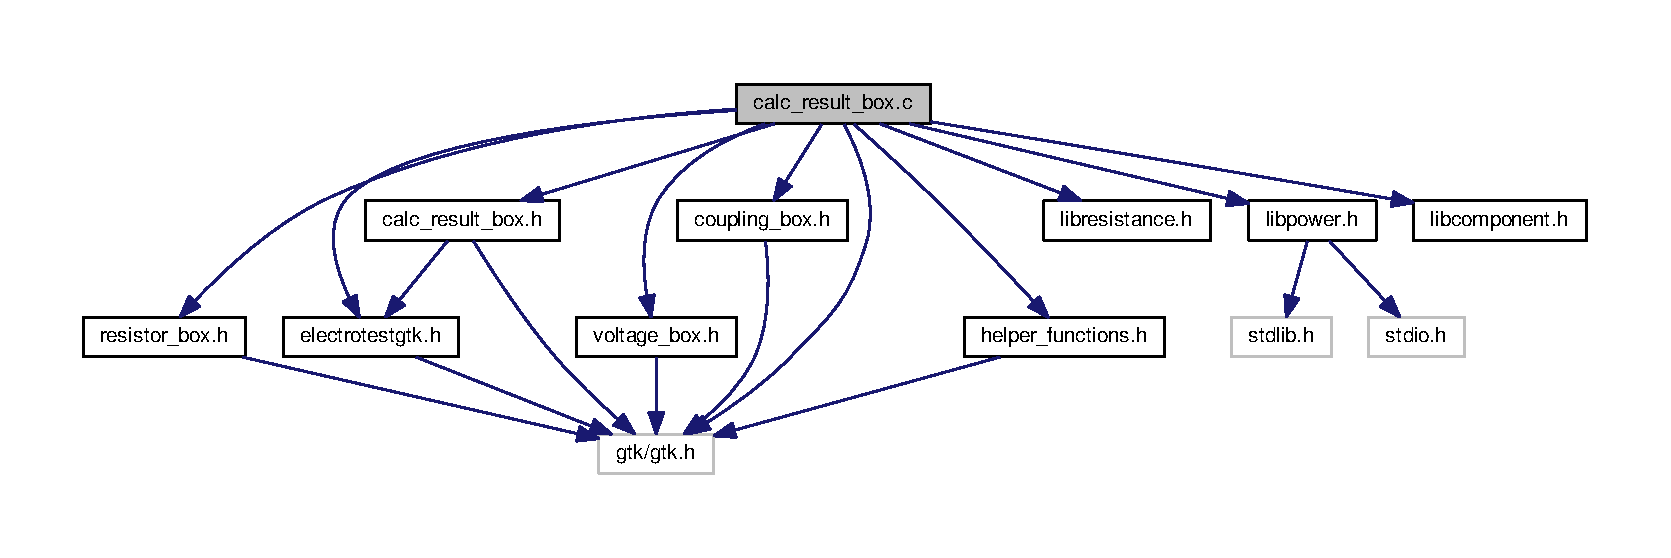
\includegraphics[width=350pt]{calc__result__box_8c__incl}
\end{center}
\end{figure}
\subsection*{Functions}
\begin{DoxyCompactItemize}
\item 
void \hyperlink{calc__result__box_8c_a4e512d25671372fda598cd3609bccad5}{button\+\_\+clicked} (Gtk\+Widget $\ast$button, struct \hyperlink{structgui__comp}{gui\+\_\+comp} $\ast$gui)
\begin{DoxyCompactList}\small\item\em callback function for calculation button \end{DoxyCompactList}\item 
Gtk\+Widget $\ast$ \hyperlink{calc__result__box_8c_acd610c39c67f9c949378aaa89cebb916}{calc\+\_\+result\+\_\+box\+\_\+new} (struct \hyperlink{structgui__comp}{gui\+\_\+comp} $\ast$gui)
\begin{DoxyCompactList}\small\item\em Constructor of the lower G\+UI part. \end{DoxyCompactList}\end{DoxyCompactItemize}
\subsection*{Variables}
\begin{DoxyCompactItemize}
\item 
Gtk\+Widget $\ast$ \hyperlink{calc__result__box_8c_a03bdde00fd1c6cf10c29b023d34a33b4}{result\+\_\+power}
\item 
Gtk\+Widget $\ast$ \hyperlink{calc__result__box_8c_a29071cefa6e04bbd40f54406d4de450f}{result\+\_\+resistance}
\end{DoxyCompactItemize}


\subsection{Function Documentation}
\index{calc\+\_\+result\+\_\+box.\+c@{calc\+\_\+result\+\_\+box.\+c}!button\+\_\+clicked@{button\+\_\+clicked}}
\index{button\+\_\+clicked@{button\+\_\+clicked}!calc\+\_\+result\+\_\+box.\+c@{calc\+\_\+result\+\_\+box.\+c}}
\subsubsection[{\texorpdfstring{button\+\_\+clicked(\+Gtk\+Widget $\ast$button, struct gui\+\_\+comp $\ast$gui)}{button_clicked(GtkWidget *button, struct gui_comp *gui)}}]{\setlength{\rightskip}{0pt plus 5cm}void button\+\_\+clicked (
\begin{DoxyParamCaption}
\item[{Gtk\+Widget $\ast$}]{button, }
\item[{struct {\bf gui\+\_\+comp} $\ast$}]{gui}
\end{DoxyParamCaption}
)}\hypertarget{calc__result__box_8c_a4e512d25671372fda598cd3609bccad5}{}\label{calc__result__box_8c_a4e512d25671372fda598cd3609bccad5}


callback function for calculation button 

Function uses the electrotest libraries to calculate the replacement resistor and power. Currently, no additional error handling over the libraries is implemented. The function takes a struct with pointers to the relevant gui parts and the data array that contains the resistor values.


\begin{DoxyParams}{Parameters}
{\em button} & The button widget to which the callback relates. \\
\hline
{\em gui} & A struct that contains pointers to all gui parts and to the array which contains the resistor values. \\
\hline
\end{DoxyParams}
\index{calc\+\_\+result\+\_\+box.\+c@{calc\+\_\+result\+\_\+box.\+c}!calc\+\_\+result\+\_\+box\+\_\+new@{calc\+\_\+result\+\_\+box\+\_\+new}}
\index{calc\+\_\+result\+\_\+box\+\_\+new@{calc\+\_\+result\+\_\+box\+\_\+new}!calc\+\_\+result\+\_\+box.\+c@{calc\+\_\+result\+\_\+box.\+c}}
\subsubsection[{\texorpdfstring{calc\+\_\+result\+\_\+box\+\_\+new(struct gui\+\_\+comp $\ast$gui)}{calc_result_box_new(struct gui_comp *gui)}}]{\setlength{\rightskip}{0pt plus 5cm}Gtk\+Widget$\ast$ calc\+\_\+result\+\_\+box\+\_\+new (
\begin{DoxyParamCaption}
\item[{struct {\bf gui\+\_\+comp} $\ast$}]{gui}
\end{DoxyParamCaption}
)}\hypertarget{calc__result__box_8c_acd610c39c67f9c949378aaa89cebb916}{}\label{calc__result__box_8c_acd610c39c67f9c949378aaa89cebb916}


Constructor of the lower G\+UI part. 

This part of the G\+UI contains the calculation button and the result boxes.


\begin{DoxyParams}{Parameters}
{\em gui} & A struct that contains pointers to all gui parts and to the array which contains the resistor values. \\
\hline
\end{DoxyParams}
\begin{DoxyReturn}{Returns}
Gtk\+Widget$\ast$ Pointer to the constructed and wired-\/up G\+UI part 
\end{DoxyReturn}


\subsection{Variable Documentation}
\index{calc\+\_\+result\+\_\+box.\+c@{calc\+\_\+result\+\_\+box.\+c}!result\+\_\+power@{result\+\_\+power}}
\index{result\+\_\+power@{result\+\_\+power}!calc\+\_\+result\+\_\+box.\+c@{calc\+\_\+result\+\_\+box.\+c}}
\subsubsection[{\texorpdfstring{result\+\_\+power}{result_power}}]{\setlength{\rightskip}{0pt plus 5cm}Gtk\+Widget$\ast$ result\+\_\+power}\hypertarget{calc__result__box_8c_a03bdde00fd1c6cf10c29b023d34a33b4}{}\label{calc__result__box_8c_a03bdde00fd1c6cf10c29b023d34a33b4}
\index{calc\+\_\+result\+\_\+box.\+c@{calc\+\_\+result\+\_\+box.\+c}!result\+\_\+resistance@{result\+\_\+resistance}}
\index{result\+\_\+resistance@{result\+\_\+resistance}!calc\+\_\+result\+\_\+box.\+c@{calc\+\_\+result\+\_\+box.\+c}}
\subsubsection[{\texorpdfstring{result\+\_\+resistance}{result_resistance}}]{\setlength{\rightskip}{0pt plus 5cm}Gtk\+Widget$\ast$ result\+\_\+resistance}\hypertarget{calc__result__box_8c_a29071cefa6e04bbd40f54406d4de450f}{}\label{calc__result__box_8c_a29071cefa6e04bbd40f54406d4de450f}

\hypertarget{calc__result__box_8h}{}\section{calc\+\_\+result\+\_\+box.\+h File Reference}
\label{calc__result__box_8h}\index{calc\+\_\+result\+\_\+box.\+h@{calc\+\_\+result\+\_\+box.\+h}}
{\ttfamily \#include $<$gtk/gtk.\+h$>$}\\*
{\ttfamily \#include \char`\"{}electrotestgtk.\+h\char`\"{}}\\*
Include dependency graph for calc\+\_\+result\+\_\+box.\+h\+:
\nopagebreak
\begin{figure}[H]
\begin{center}
\leavevmode
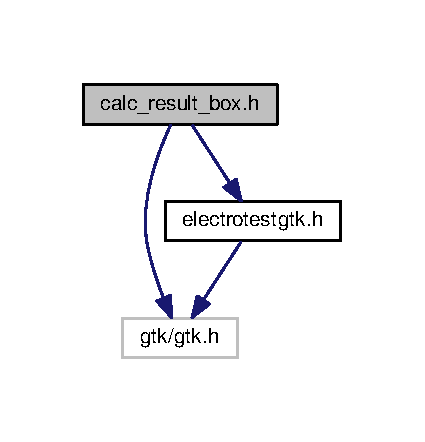
\includegraphics[width=204pt]{calc__result__box_8h__incl}
\end{center}
\end{figure}
This graph shows which files directly or indirectly include this file\+:
\nopagebreak
\begin{figure}[H]
\begin{center}
\leavevmode
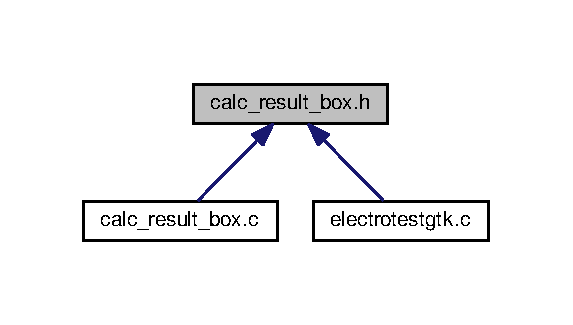
\includegraphics[width=275pt]{calc__result__box_8h__dep__incl}
\end{center}
\end{figure}
\subsection*{Functions}
\begin{DoxyCompactItemize}
\item 
Gtk\+Widget $\ast$ \hyperlink{calc__result__box_8h_acd610c39c67f9c949378aaa89cebb916}{calc\+\_\+result\+\_\+box\+\_\+new} (struct \hyperlink{structgui__comp}{gui\+\_\+comp} $\ast$gui)
\begin{DoxyCompactList}\small\item\em Constructor of the lower G\+UI part. \end{DoxyCompactList}\end{DoxyCompactItemize}


\subsection{Function Documentation}
\index{calc\+\_\+result\+\_\+box.\+h@{calc\+\_\+result\+\_\+box.\+h}!calc\+\_\+result\+\_\+box\+\_\+new@{calc\+\_\+result\+\_\+box\+\_\+new}}
\index{calc\+\_\+result\+\_\+box\+\_\+new@{calc\+\_\+result\+\_\+box\+\_\+new}!calc\+\_\+result\+\_\+box.\+h@{calc\+\_\+result\+\_\+box.\+h}}
\subsubsection[{\texorpdfstring{calc\+\_\+result\+\_\+box\+\_\+new(struct gui\+\_\+comp $\ast$gui)}{calc_result_box_new(struct gui_comp *gui)}}]{\setlength{\rightskip}{0pt plus 5cm}Gtk\+Widget$\ast$ calc\+\_\+result\+\_\+box\+\_\+new (
\begin{DoxyParamCaption}
\item[{struct {\bf gui\+\_\+comp} $\ast$}]{gui}
\end{DoxyParamCaption}
)}\hypertarget{calc__result__box_8h_acd610c39c67f9c949378aaa89cebb916}{}\label{calc__result__box_8h_acd610c39c67f9c949378aaa89cebb916}


Constructor of the lower G\+UI part. 

This part of the G\+UI contains the calculation button and the result boxes.


\begin{DoxyParams}{Parameters}
{\em gui} & A struct that contains pointers to all gui parts and to the array which contains the resistor values. \\
\hline
\end{DoxyParams}
\begin{DoxyReturn}{Returns}
calc\+\_\+result\+\_\+box The constructed and wired G\+UI part
\end{DoxyReturn}
This part of the G\+UI contains the calculation button and the result boxes.


\begin{DoxyParams}{Parameters}
{\em gui} & A struct that contains pointers to all gui parts and to the array which contains the resistor values. \\
\hline
\end{DoxyParams}
\begin{DoxyReturn}{Returns}
Gtk\+Widget$\ast$ Pointer to the constructed and wired-\/up G\+UI part 
\end{DoxyReturn}

\hypertarget{coupling__box_8c}{}\section{coupling\+\_\+box.\+c File Reference}
\label{coupling__box_8c}\index{coupling\+\_\+box.\+c@{coupling\+\_\+box.\+c}}
{\ttfamily \#include $<$gtk/gtk.\+h$>$}\\*
{\ttfamily \#include \char`\"{}coupling\+\_\+box.\+h\char`\"{}}\\*
{\ttfamily \#include \char`\"{}helper\+\_\+functions.\+h\char`\"{}}\\*
Include dependency graph for coupling\+\_\+box.\+c\+:
\nopagebreak
\begin{figure}[H]
\begin{center}
\leavevmode
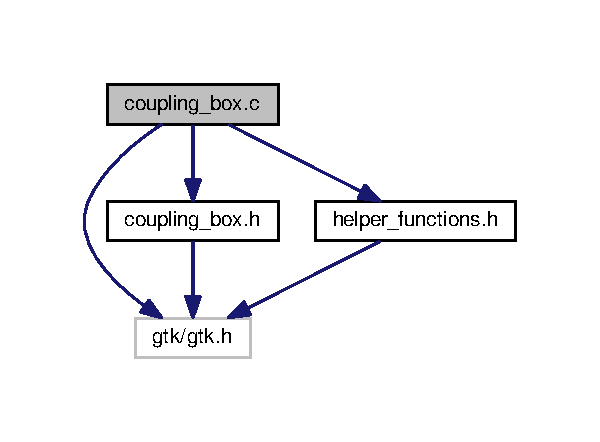
\includegraphics[width=288pt]{coupling__box_8c__incl}
\end{center}
\end{figure}
\subsection*{Functions}
\begin{DoxyCompactItemize}
\item 
Gtk\+Widget $\ast$ \hyperlink{coupling__box_8c_a76dc11e43bebffd131ce50fdf01027b6}{coupling\+\_\+box\+\_\+new} (void)
\begin{DoxyCompactList}\small\item\em Constructor for the Resistor Coupling Gui part. \end{DoxyCompactList}\item 
int \hyperlink{coupling__box_8c_a38db3eb6757a718a47ddb339f5b15bd4}{get\+\_\+coupling} (Gtk\+Widget $\ast$coupling\+\_\+box)
\begin{DoxyCompactList}\small\item\em Getter for mode of resistor coupling. \end{DoxyCompactList}\end{DoxyCompactItemize}


\subsection{Function Documentation}
\index{coupling\+\_\+box.\+c@{coupling\+\_\+box.\+c}!coupling\+\_\+box\+\_\+new@{coupling\+\_\+box\+\_\+new}}
\index{coupling\+\_\+box\+\_\+new@{coupling\+\_\+box\+\_\+new}!coupling\+\_\+box.\+c@{coupling\+\_\+box.\+c}}
\subsubsection[{\texorpdfstring{coupling\+\_\+box\+\_\+new(void)}{coupling_box_new(void)}}]{\setlength{\rightskip}{0pt plus 5cm}Gtk\+Widget$\ast$ coupling\+\_\+box\+\_\+new (
\begin{DoxyParamCaption}
\item[{void}]{}
\end{DoxyParamCaption}
)}\hypertarget{coupling__box_8c_a76dc11e43bebffd131ce50fdf01027b6}{}\label{coupling__box_8c_a76dc11e43bebffd131ce50fdf01027b6}


Constructor for the Resistor Coupling Gui part. 

The Resistor coupling G\+UI part allows to choose between serial/parallel coupling of the resistors.

\begin{DoxyReturn}{Returns}
Gtk\+Widget$\ast$ pointer to the new created Gui part. 
\end{DoxyReturn}
\index{coupling\+\_\+box.\+c@{coupling\+\_\+box.\+c}!get\+\_\+coupling@{get\+\_\+coupling}}
\index{get\+\_\+coupling@{get\+\_\+coupling}!coupling\+\_\+box.\+c@{coupling\+\_\+box.\+c}}
\subsubsection[{\texorpdfstring{get\+\_\+coupling(\+Gtk\+Widget $\ast$coupling\+\_\+box)}{get_coupling(GtkWidget *coupling_box)}}]{\setlength{\rightskip}{0pt plus 5cm}int get\+\_\+coupling (
\begin{DoxyParamCaption}
\item[{Gtk\+Widget $\ast$}]{coupling\+\_\+box}
\end{DoxyParamCaption}
)}\hypertarget{coupling__box_8c_a38db3eb6757a718a47ddb339f5b15bd4}{}\label{coupling__box_8c_a38db3eb6757a718a47ddb339f5b15bd4}


Getter for mode of resistor coupling. 

Function that queries the selected resitor coupling mode in the gui and returns 1 for serial and 0 for parallel.

\begin{DoxyReturn}{Returns}
1 = serial, 0 = parallel 
\end{DoxyReturn}

\hypertarget{coupling__box_8h}{}\section{coupling\+\_\+box.\+h File Reference}
\label{coupling__box_8h}\index{coupling\+\_\+box.\+h@{coupling\+\_\+box.\+h}}
{\ttfamily \#include $<$gtk/gtk.\+h$>$}\\*
Include dependency graph for coupling\+\_\+box.\+h\+:
\nopagebreak
\begin{figure}[H]
\begin{center}
\leavevmode
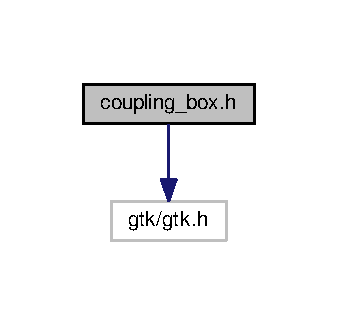
\includegraphics[width=162pt]{coupling__box_8h__incl}
\end{center}
\end{figure}
This graph shows which files directly or indirectly include this file\+:
\nopagebreak
\begin{figure}[H]
\begin{center}
\leavevmode
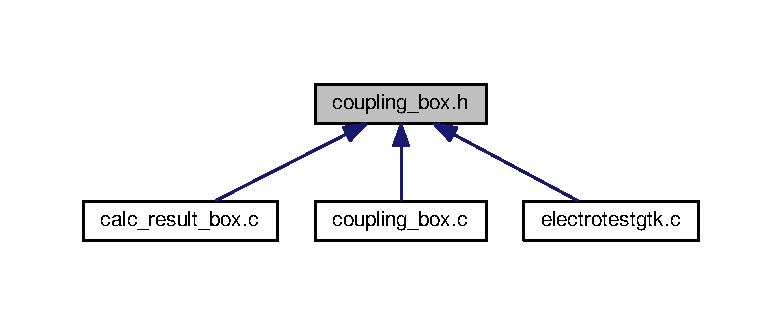
\includegraphics[width=350pt]{coupling__box_8h__dep__incl}
\end{center}
\end{figure}
\subsection*{Functions}
\begin{DoxyCompactItemize}
\item 
Gtk\+Widget $\ast$ \hyperlink{coupling__box_8h_a76dc11e43bebffd131ce50fdf01027b6}{coupling\+\_\+box\+\_\+new} (void)
\begin{DoxyCompactList}\small\item\em Constructor for the Resistor Coupling Gui part. \end{DoxyCompactList}\item 
int \hyperlink{coupling__box_8h_a38db3eb6757a718a47ddb339f5b15bd4}{get\+\_\+coupling} (Gtk\+Widget $\ast$coupling\+\_\+box)
\begin{DoxyCompactList}\small\item\em Getter for mode of resistor coupling. \end{DoxyCompactList}\end{DoxyCompactItemize}


\subsection{Function Documentation}
\index{coupling\+\_\+box.\+h@{coupling\+\_\+box.\+h}!coupling\+\_\+box\+\_\+new@{coupling\+\_\+box\+\_\+new}}
\index{coupling\+\_\+box\+\_\+new@{coupling\+\_\+box\+\_\+new}!coupling\+\_\+box.\+h@{coupling\+\_\+box.\+h}}
\subsubsection[{\texorpdfstring{coupling\+\_\+box\+\_\+new(void)}{coupling_box_new(void)}}]{\setlength{\rightskip}{0pt plus 5cm}Gtk\+Widget$\ast$ coupling\+\_\+box\+\_\+new (
\begin{DoxyParamCaption}
\item[{void}]{}
\end{DoxyParamCaption}
)}\hypertarget{coupling__box_8h_a76dc11e43bebffd131ce50fdf01027b6}{}\label{coupling__box_8h_a76dc11e43bebffd131ce50fdf01027b6}


Constructor for the Resistor Coupling Gui part. 

The Resistor coupling G\+UI part allows to choose between serial/parallel coupling of the resistors.

\begin{DoxyReturn}{Returns}
Gtk\+Widget$\ast$ pointer to the new created Gui part. 
\end{DoxyReturn}
\index{coupling\+\_\+box.\+h@{coupling\+\_\+box.\+h}!get\+\_\+coupling@{get\+\_\+coupling}}
\index{get\+\_\+coupling@{get\+\_\+coupling}!coupling\+\_\+box.\+h@{coupling\+\_\+box.\+h}}
\subsubsection[{\texorpdfstring{get\+\_\+coupling(\+Gtk\+Widget $\ast$coupling\+\_\+box)}{get_coupling(GtkWidget *coupling_box)}}]{\setlength{\rightskip}{0pt plus 5cm}int get\+\_\+coupling (
\begin{DoxyParamCaption}
\item[{Gtk\+Widget $\ast$}]{coupling\+\_\+box}
\end{DoxyParamCaption}
)}\hypertarget{coupling__box_8h_a38db3eb6757a718a47ddb339f5b15bd4}{}\label{coupling__box_8h_a38db3eb6757a718a47ddb339f5b15bd4}


Getter for mode of resistor coupling. 

Function that queries the selected resitor coupling mode in the gui and returns 1 for serial and 0 for parallel.

\begin{DoxyReturn}{Returns}
1 = serial, 0 = parallel 
\end{DoxyReturn}

\hypertarget{electrotestgtk_8c}{}\section{electrotestgtk.\+c File Reference}
\label{electrotestgtk_8c}\index{electrotestgtk.\+c@{electrotestgtk.\+c}}
{\ttfamily \#include $<$gtk/gtk.\+h$>$}\\*
{\ttfamily \#include $<$stdio.\+h$>$}\\*
{\ttfamily \#include $<$string.\+h$>$}\\*
{\ttfamily \#include \char`\"{}electrotestgtk.\+h\char`\"{}}\\*
{\ttfamily \#include \char`\"{}voltage\+\_\+box.\+h\char`\"{}}\\*
{\ttfamily \#include \char`\"{}resistor\+\_\+box.\+h\char`\"{}}\\*
{\ttfamily \#include \char`\"{}coupling\+\_\+box.\+h\char`\"{}}\\*
{\ttfamily \#include \char`\"{}calc\+\_\+result\+\_\+box.\+h\char`\"{}}\\*
{\ttfamily \#include \char`\"{}helper\+\_\+functions.\+h\char`\"{}}\\*
{\ttfamily \#include \char`\"{}libresistance.\+h\char`\"{}}\\*
{\ttfamily \#include \char`\"{}libpower.\+h\char`\"{}}\\*
{\ttfamily \#include \char`\"{}libcomponent.\+h\char`\"{}}\\*
Include dependency graph for electrotestgtk.\+c\+:
\nopagebreak
\begin{figure}[H]
\begin{center}
\leavevmode
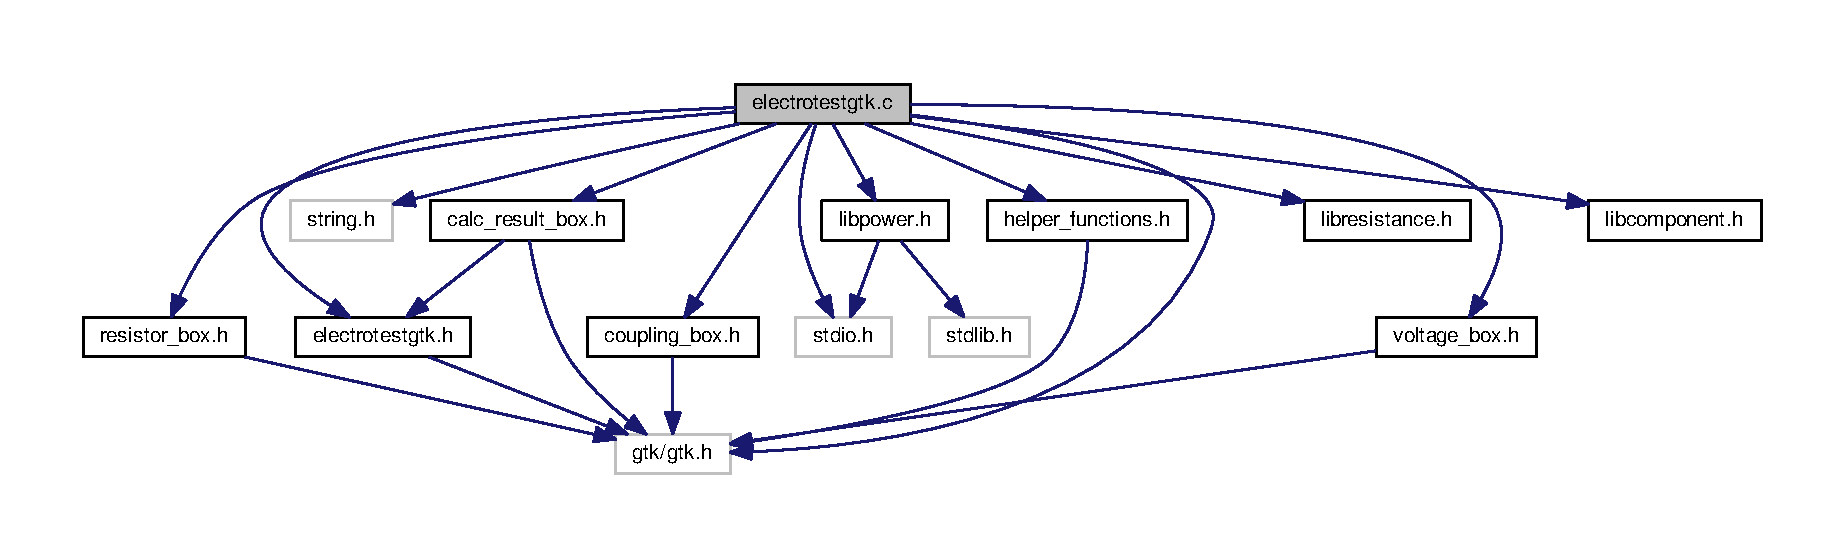
\includegraphics[width=350pt]{electrotestgtk_8c__incl}
\end{center}
\end{figure}
\subsection*{Functions}
\begin{DoxyCompactItemize}
\item 
void \hyperlink{electrotestgtk_8c_a7ec75a115453b506dbd31c4675a206f1}{close\+App} (Gtk\+Widget $\ast$window, gpointer data)
\begin{DoxyCompactList}\small\item\em close\+App callback function \end{DoxyCompactList}\item 
gint \hyperlink{electrotestgtk_8c_a7490dccd8cae3e56d4df21f6d03c351d}{main} (gint argc, gchar $\ast$argv\mbox{[}$\,$\mbox{]})
\begin{DoxyCompactList}\small\item\em Main of electrotestgtk Application. \end{DoxyCompactList}\end{DoxyCompactItemize}


\subsection{Function Documentation}
\index{electrotestgtk.\+c@{electrotestgtk.\+c}!close\+App@{close\+App}}
\index{close\+App@{close\+App}!electrotestgtk.\+c@{electrotestgtk.\+c}}
\subsubsection[{\texorpdfstring{close\+App(\+Gtk\+Widget $\ast$window, gpointer data)}{closeApp(GtkWidget *window, gpointer data)}}]{\setlength{\rightskip}{0pt plus 5cm}void close\+App (
\begin{DoxyParamCaption}
\item[{Gtk\+Widget $\ast$}]{window, }
\item[{gpointer}]{data}
\end{DoxyParamCaption}
)}\hypertarget{electrotestgtk_8c_a7ec75a115453b506dbd31c4675a206f1}{}\label{electrotestgtk_8c_a7ec75a115453b506dbd31c4675a206f1}


close\+App callback function 

Function to close main G\+TK application window.


\begin{DoxyParams}{Parameters}
{\em window,pointer} & to the main window widget \\
\hline
{\em data,pointer} & for extra data, not used \\
\hline
\end{DoxyParams}
\index{electrotestgtk.\+c@{electrotestgtk.\+c}!main@{main}}
\index{main@{main}!electrotestgtk.\+c@{electrotestgtk.\+c}}
\subsubsection[{\texorpdfstring{main(gint argc, gchar $\ast$argv[])}{main(gint argc, gchar *argv[])}}]{\setlength{\rightskip}{0pt plus 5cm}gint main (
\begin{DoxyParamCaption}
\item[{gint}]{argc, }
\item[{gchar $\ast$}]{argv\mbox{[}$\,$\mbox{]}}
\end{DoxyParamCaption}
)}\hypertarget{electrotestgtk_8c_a7490dccd8cae3e56d4df21f6d03c351d}{}\label{electrotestgtk_8c_a7490dccd8cae3e56d4df21f6d03c351d}


Main of electrotestgtk Application. 

Application G\+T\+K+ gui frontend for electrotest libraries. The Main file constructs the G\+UI by calling the three respective constructor functions. Interfacing to the libraries happens mostly in the calc\+\_\+results\+\_\+box gui part. Currently the application does not implement advanced user input validation and relies on the functionality in the libraries. $\ast$ 
\hypertarget{electrotestgtk_8h}{}\section{electrotestgtk.\+h File Reference}
\label{electrotestgtk_8h}\index{electrotestgtk.\+h@{electrotestgtk.\+h}}
{\ttfamily \#include $<$gtk/gtk.\+h$>$}\\*
Include dependency graph for electrotestgtk.\+h\+:
\nopagebreak
\begin{figure}[H]
\begin{center}
\leavevmode
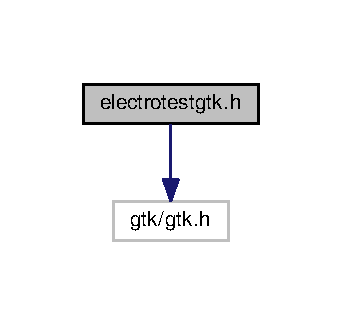
\includegraphics[width=164pt]{electrotestgtk_8h__incl}
\end{center}
\end{figure}
This graph shows which files directly or indirectly include this file\+:
\nopagebreak
\begin{figure}[H]
\begin{center}
\leavevmode
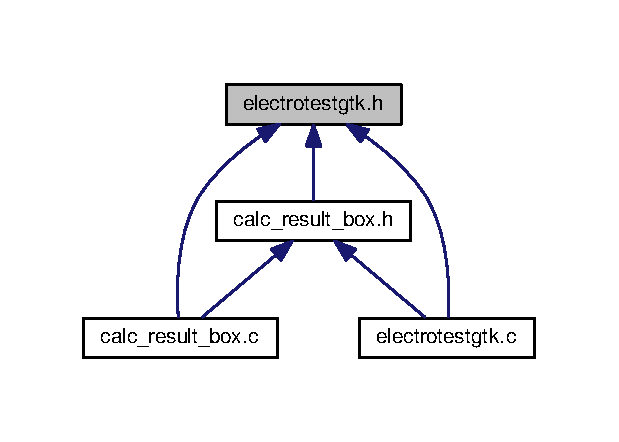
\includegraphics[width=297pt]{electrotestgtk_8h__dep__incl}
\end{center}
\end{figure}
\subsection*{Data Structures}
\begin{DoxyCompactItemize}
\item 
struct \hyperlink{structgui__comp}{gui\+\_\+comp}
\begin{DoxyCompactList}\small\item\em Struct with pointers to all gui and data parts. \end{DoxyCompactList}\end{DoxyCompactItemize}

\hypertarget{helper__functions_8c}{}\section{helper\+\_\+functions.\+c File Reference}
\label{helper__functions_8c}\index{helper\+\_\+functions.\+c@{helper\+\_\+functions.\+c}}
{\ttfamily \#include $<$gtk/gtk.\+h$>$}\\*
{\ttfamily \#include \char`\"{}helper\+\_\+functions.\+h\char`\"{}}\\*
Include dependency graph for helper\+\_\+functions.\+c\+:
\nopagebreak
\begin{figure}[H]
\begin{center}
\leavevmode
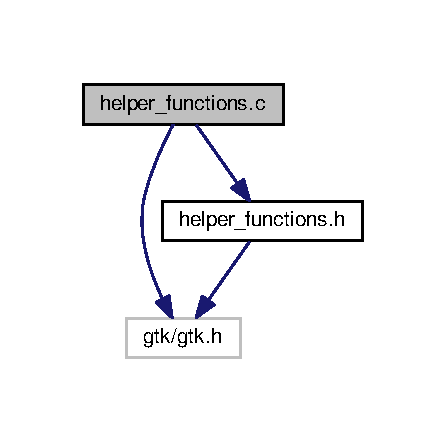
\includegraphics[width=214pt]{helper__functions_8c__incl}
\end{center}
\end{figure}
\subsection*{Functions}
\begin{DoxyCompactItemize}
\item 
Gtk\+Widget $\ast$ \hyperlink{helper__functions_8c_af86dd601bf334aeed93cb1622cffdc52}{add\+\_\+widget\+\_\+with\+\_\+label\+\_\+vbox} (Gtk\+Container $\ast$box, gchar $\ast$caption, Gtk\+Widget $\ast$widget)
\begin{DoxyCompactList}\small\item\em Function constructs a label above a provided widget. \end{DoxyCompactList}\item 
Gtk\+Widget $\ast$ \hyperlink{helper__functions_8c_a3fbd1d54b640d4111a474a0ba2578f68}{add\+\_\+widget\+\_\+with\+\_\+label\+\_\+hbox} (Gtk\+Container $\ast$box, gchar $\ast$caption, Gtk\+Widget $\ast$widget)
\begin{DoxyCompactList}\small\item\em Function constructs a label to the left of a provided widget. \end{DoxyCompactList}\item 
Gtk\+Widget $\ast$ \hyperlink{helper__functions_8c_a979e4c6c8f0994dd482867c9c5db4c99}{gtk\+\_\+entry\+\_\+with\+\_\+name\+\_\+new} (gchar $\ast$name)
\begin{DoxyCompactList}\small\item\em Helper to create entry widget with a name. \end{DoxyCompactList}\item 
Gtk\+Widget $\ast$ \hyperlink{helper__functions_8c_ac0b769c1ba8b9da1aadd11681c5d3eee}{find\+\_\+child} (Gtk\+Widget $\ast$parent, const gchar $\ast$name)
\begin{DoxyCompactList}\small\item\em Find recursively child widgets of a G\+TK container by name. \end{DoxyCompactList}\end{DoxyCompactItemize}


\subsection{Function Documentation}
\index{helper\+\_\+functions.\+c@{helper\+\_\+functions.\+c}!add\+\_\+widget\+\_\+with\+\_\+label\+\_\+hbox@{add\+\_\+widget\+\_\+with\+\_\+label\+\_\+hbox}}
\index{add\+\_\+widget\+\_\+with\+\_\+label\+\_\+hbox@{add\+\_\+widget\+\_\+with\+\_\+label\+\_\+hbox}!helper\+\_\+functions.\+c@{helper\+\_\+functions.\+c}}
\subsubsection[{\texorpdfstring{add\+\_\+widget\+\_\+with\+\_\+label\+\_\+hbox(\+Gtk\+Container $\ast$box, gchar $\ast$caption, Gtk\+Widget $\ast$widget)}{add_widget_with_label_hbox(GtkContainer *box, gchar *caption, GtkWidget *widget)}}]{\setlength{\rightskip}{0pt plus 5cm}Gtk\+Widget$\ast$ add\+\_\+widget\+\_\+with\+\_\+label\+\_\+hbox (
\begin{DoxyParamCaption}
\item[{Gtk\+Container $\ast$}]{box, }
\item[{gchar $\ast$}]{caption, }
\item[{Gtk\+Widget $\ast$}]{widget}
\end{DoxyParamCaption}
)}\hypertarget{helper__functions_8c_a3fbd1d54b640d4111a474a0ba2578f68}{}\label{helper__functions_8c_a3fbd1d54b640d4111a474a0ba2578f68}


Function constructs a label to the left of a provided widget. 

The function creates a new hbox and a label. The provided widget is put in the hbox together with the new label which results in a label to the left of the widget. The hbox is then put into the provided container/box.


\begin{DoxyParams}{Parameters}
{\em box} & Gtk Container into which the hbox with label and widget shall be added \\
\hline
{\em caption} & String used to construct the caption \\
\hline
{\em widget} & widget to which a label shall be constructed \\
\hline
\end{DoxyParams}
\begin{DoxyReturn}{Returns}
Gtk\+Widget$\ast$ returns pointer to the given box/container. This is not always needed but sometimes of advantage when multiple widgets shall be constructed in a loop with a deeply nested constructor. 
\end{DoxyReturn}
\index{helper\+\_\+functions.\+c@{helper\+\_\+functions.\+c}!add\+\_\+widget\+\_\+with\+\_\+label\+\_\+vbox@{add\+\_\+widget\+\_\+with\+\_\+label\+\_\+vbox}}
\index{add\+\_\+widget\+\_\+with\+\_\+label\+\_\+vbox@{add\+\_\+widget\+\_\+with\+\_\+label\+\_\+vbox}!helper\+\_\+functions.\+c@{helper\+\_\+functions.\+c}}
\subsubsection[{\texorpdfstring{add\+\_\+widget\+\_\+with\+\_\+label\+\_\+vbox(\+Gtk\+Container $\ast$box, gchar $\ast$caption, Gtk\+Widget $\ast$widget)}{add_widget_with_label_vbox(GtkContainer *box, gchar *caption, GtkWidget *widget)}}]{\setlength{\rightskip}{0pt plus 5cm}Gtk\+Widget$\ast$ add\+\_\+widget\+\_\+with\+\_\+label\+\_\+vbox (
\begin{DoxyParamCaption}
\item[{Gtk\+Container $\ast$}]{box, }
\item[{gchar $\ast$}]{caption, }
\item[{Gtk\+Widget $\ast$}]{widget}
\end{DoxyParamCaption}
)}\hypertarget{helper__functions_8c_af86dd601bf334aeed93cb1622cffdc52}{}\label{helper__functions_8c_af86dd601bf334aeed93cb1622cffdc52}


Function constructs a label above a provided widget. 

The function creates a new vbox and a label. The provided widget is put in the vbox together with the new label which results in a label above the widget. The vbox is then put into the provided container/box.


\begin{DoxyParams}{Parameters}
{\em box} & Gtk Container into which the vbox with label and widget shall be added \\
\hline
{\em caption} & String used to construct the caption \\
\hline
{\em widget} & widget to which a label shall be constructed \\
\hline
\end{DoxyParams}
\begin{DoxyReturn}{Returns}
Gtk\+Widget$\ast$ returns pointer to the given box/container. This is not always needed but sometimes of advantage when multiple widgets shall be constructed in a loop with a deeply nested constructor. 
\end{DoxyReturn}
\index{helper\+\_\+functions.\+c@{helper\+\_\+functions.\+c}!find\+\_\+child@{find\+\_\+child}}
\index{find\+\_\+child@{find\+\_\+child}!helper\+\_\+functions.\+c@{helper\+\_\+functions.\+c}}
\subsubsection[{\texorpdfstring{find\+\_\+child(\+Gtk\+Widget $\ast$parent, const gchar $\ast$name)}{find_child(GtkWidget *parent, const gchar *name)}}]{\setlength{\rightskip}{0pt plus 5cm}Gtk\+Widget$\ast$ find\+\_\+child (
\begin{DoxyParamCaption}
\item[{Gtk\+Widget $\ast$}]{parent, }
\item[{const gchar $\ast$}]{name}
\end{DoxyParamCaption}
)}\hypertarget{helper__functions_8c_ac0b769c1ba8b9da1aadd11681c5d3eee}{}\label{helper__functions_8c_ac0b769c1ba8b9da1aadd11681c5d3eee}


Find recursively child widgets of a G\+TK container by name. 

Recursive search of child widgets in a G\+TK container structure. The function returns, when found a pointer to the respective widget, else N\+U\+LL. 
\begin{DoxyParams}{Parameters}
{\em parent} & Widget to start the search at. \\
\hline
{\em name} & String of the name to search for \\
\hline
\end{DoxyParams}
\begin{DoxyReturn}{Returns}
pointer to the found widget or N\+U\+LL 
\end{DoxyReturn}
\index{helper\+\_\+functions.\+c@{helper\+\_\+functions.\+c}!gtk\+\_\+entry\+\_\+with\+\_\+name\+\_\+new@{gtk\+\_\+entry\+\_\+with\+\_\+name\+\_\+new}}
\index{gtk\+\_\+entry\+\_\+with\+\_\+name\+\_\+new@{gtk\+\_\+entry\+\_\+with\+\_\+name\+\_\+new}!helper\+\_\+functions.\+c@{helper\+\_\+functions.\+c}}
\subsubsection[{\texorpdfstring{gtk\+\_\+entry\+\_\+with\+\_\+name\+\_\+new(gchar $\ast$name)}{gtk_entry_with_name_new(gchar *name)}}]{\setlength{\rightskip}{0pt plus 5cm}Gtk\+Widget$\ast$ gtk\+\_\+entry\+\_\+with\+\_\+name\+\_\+new (
\begin{DoxyParamCaption}
\item[{gchar $\ast$}]{name}
\end{DoxyParamCaption}
)}\hypertarget{helper__functions_8c_a979e4c6c8f0994dd482867c9c5db4c99}{}\label{helper__functions_8c_a979e4c6c8f0994dd482867c9c5db4c99}


Helper to create entry widget with a name. 

Naming widgets is handy as they can be searched easily with \hyperlink{helper__functions_8c_ac0b769c1ba8b9da1aadd11681c5d3eee}{find\+\_\+child()} also provided in this helper function collection.


\begin{DoxyParams}{Parameters}
{\em name} & string on how to name the new entry widget \\
\hline
\end{DoxyParams}
\begin{DoxyReturn}{Returns}
Gtk\+Widget$\ast$ pointer to the constructed and named gtk\+\_\+entry widget 
\end{DoxyReturn}

\hypertarget{helper__functions_8h}{}\section{helper\+\_\+functions.\+h File Reference}
\label{helper__functions_8h}\index{helper\+\_\+functions.\+h@{helper\+\_\+functions.\+h}}
{\ttfamily \#include $<$gtk/gtk.\+h$>$}\\*
Include dependency graph for helper\+\_\+functions.\+h\+:
\nopagebreak
\begin{figure}[H]
\begin{center}
\leavevmode
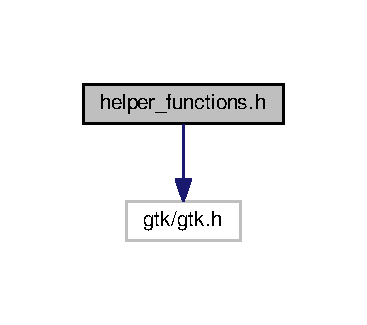
\includegraphics[width=176pt]{helper__functions_8h__incl}
\end{center}
\end{figure}
This graph shows which files directly or indirectly include this file\+:
\nopagebreak
\begin{figure}[H]
\begin{center}
\leavevmode
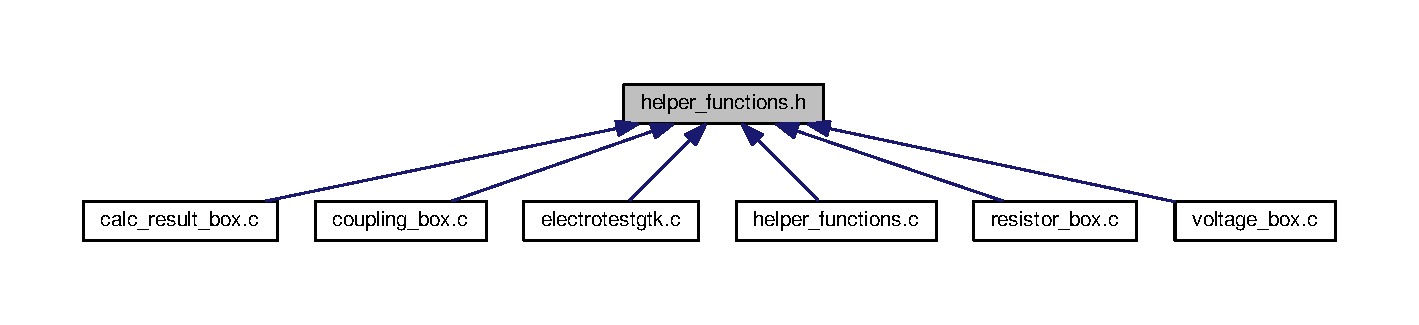
\includegraphics[width=350pt]{helper__functions_8h__dep__incl}
\end{center}
\end{figure}
\subsection*{Functions}
\begin{DoxyCompactItemize}
\item 
Gtk\+Widget $\ast$ \hyperlink{helper__functions_8h_af86dd601bf334aeed93cb1622cffdc52}{add\+\_\+widget\+\_\+with\+\_\+label\+\_\+vbox} (Gtk\+Container $\ast$box, gchar $\ast$caption, Gtk\+Widget $\ast$widget)
\begin{DoxyCompactList}\small\item\em Function constructs a label above a provided widget. \end{DoxyCompactList}\item 
Gtk\+Widget $\ast$ \hyperlink{helper__functions_8h_a3fbd1d54b640d4111a474a0ba2578f68}{add\+\_\+widget\+\_\+with\+\_\+label\+\_\+hbox} (Gtk\+Container $\ast$box, gchar $\ast$caption, Gtk\+Widget $\ast$widget)
\begin{DoxyCompactList}\small\item\em Function constructs a label to the left of a provided widget. \end{DoxyCompactList}\item 
Gtk\+Widget $\ast$ \hyperlink{helper__functions_8h_ac0b769c1ba8b9da1aadd11681c5d3eee}{find\+\_\+child} (Gtk\+Widget $\ast$parent, const gchar $\ast$name)
\begin{DoxyCompactList}\small\item\em Find recursively child widgets of a G\+TK container by name. \end{DoxyCompactList}\item 
Gtk\+Widget $\ast$ \hyperlink{helper__functions_8h_a979e4c6c8f0994dd482867c9c5db4c99}{gtk\+\_\+entry\+\_\+with\+\_\+name\+\_\+new} (gchar $\ast$name)
\begin{DoxyCompactList}\small\item\em Helper to create entry widget with a name. \end{DoxyCompactList}\end{DoxyCompactItemize}


\subsection{Function Documentation}
\index{helper\+\_\+functions.\+h@{helper\+\_\+functions.\+h}!add\+\_\+widget\+\_\+with\+\_\+label\+\_\+hbox@{add\+\_\+widget\+\_\+with\+\_\+label\+\_\+hbox}}
\index{add\+\_\+widget\+\_\+with\+\_\+label\+\_\+hbox@{add\+\_\+widget\+\_\+with\+\_\+label\+\_\+hbox}!helper\+\_\+functions.\+h@{helper\+\_\+functions.\+h}}
\subsubsection[{\texorpdfstring{add\+\_\+widget\+\_\+with\+\_\+label\+\_\+hbox(\+Gtk\+Container $\ast$box, gchar $\ast$caption, Gtk\+Widget $\ast$widget)}{add_widget_with_label_hbox(GtkContainer *box, gchar *caption, GtkWidget *widget)}}]{\setlength{\rightskip}{0pt plus 5cm}Gtk\+Widget$\ast$ add\+\_\+widget\+\_\+with\+\_\+label\+\_\+hbox (
\begin{DoxyParamCaption}
\item[{Gtk\+Container $\ast$}]{box, }
\item[{gchar $\ast$}]{caption, }
\item[{Gtk\+Widget $\ast$}]{widget}
\end{DoxyParamCaption}
)}\hypertarget{helper__functions_8h_a3fbd1d54b640d4111a474a0ba2578f68}{}\label{helper__functions_8h_a3fbd1d54b640d4111a474a0ba2578f68}


Function constructs a label to the left of a provided widget. 

The function creates a new hbox and a label. The provided widget is put in the hbox together with the new label which results in a label to the left of the widget. The hbox is then put into the provided container/box.


\begin{DoxyParams}{Parameters}
{\em box} & Gtk Container into which the hbox with label and widget shall be added \\
\hline
{\em caption} & String used to construct the caption \\
\hline
{\em widget} & widget to which a label shall be constructed \\
\hline
\end{DoxyParams}
\begin{DoxyReturn}{Returns}
Gtk\+Widget$\ast$ returns pointer to the given box/container. This is not always needed but sometimes of advantage when multiple widgets shall be constructed in a loop with a deeply nested constructor. 
\end{DoxyReturn}
\index{helper\+\_\+functions.\+h@{helper\+\_\+functions.\+h}!add\+\_\+widget\+\_\+with\+\_\+label\+\_\+vbox@{add\+\_\+widget\+\_\+with\+\_\+label\+\_\+vbox}}
\index{add\+\_\+widget\+\_\+with\+\_\+label\+\_\+vbox@{add\+\_\+widget\+\_\+with\+\_\+label\+\_\+vbox}!helper\+\_\+functions.\+h@{helper\+\_\+functions.\+h}}
\subsubsection[{\texorpdfstring{add\+\_\+widget\+\_\+with\+\_\+label\+\_\+vbox(\+Gtk\+Container $\ast$box, gchar $\ast$caption, Gtk\+Widget $\ast$widget)}{add_widget_with_label_vbox(GtkContainer *box, gchar *caption, GtkWidget *widget)}}]{\setlength{\rightskip}{0pt plus 5cm}Gtk\+Widget$\ast$ add\+\_\+widget\+\_\+with\+\_\+label\+\_\+vbox (
\begin{DoxyParamCaption}
\item[{Gtk\+Container $\ast$}]{box, }
\item[{gchar $\ast$}]{caption, }
\item[{Gtk\+Widget $\ast$}]{widget}
\end{DoxyParamCaption}
)}\hypertarget{helper__functions_8h_af86dd601bf334aeed93cb1622cffdc52}{}\label{helper__functions_8h_af86dd601bf334aeed93cb1622cffdc52}


Function constructs a label above a provided widget. 

The function creates a new vbox and a label. The provided widget is put in the vbox together with the new label which results in a label above the widget. The vbox is then put into the provided container/box.


\begin{DoxyParams}{Parameters}
{\em box} & Gtk Container into which the vbox with label and widget shall be added \\
\hline
{\em caption} & String used to construct the caption \\
\hline
{\em widget} & widget to which a label shall be constructed \\
\hline
\end{DoxyParams}
\begin{DoxyReturn}{Returns}
Gtk\+Widget$\ast$ returns pointer to the given box/container. This is not always needed but sometimes of advantage when multiple widgets shall be constructed in a loop with a deeply nested constructor. 
\end{DoxyReturn}
\index{helper\+\_\+functions.\+h@{helper\+\_\+functions.\+h}!find\+\_\+child@{find\+\_\+child}}
\index{find\+\_\+child@{find\+\_\+child}!helper\+\_\+functions.\+h@{helper\+\_\+functions.\+h}}
\subsubsection[{\texorpdfstring{find\+\_\+child(\+Gtk\+Widget $\ast$parent, const gchar $\ast$name)}{find_child(GtkWidget *parent, const gchar *name)}}]{\setlength{\rightskip}{0pt plus 5cm}Gtk\+Widget$\ast$ find\+\_\+child (
\begin{DoxyParamCaption}
\item[{Gtk\+Widget $\ast$}]{parent, }
\item[{const gchar $\ast$}]{name}
\end{DoxyParamCaption}
)}\hypertarget{helper__functions_8h_ac0b769c1ba8b9da1aadd11681c5d3eee}{}\label{helper__functions_8h_ac0b769c1ba8b9da1aadd11681c5d3eee}


Find recursively child widgets of a G\+TK container by name. 

Recursive search of child widgets in a G\+TK container structure. The function returns, when found a pointer to the respective widget, else N\+U\+LL. 
\begin{DoxyParams}{Parameters}
{\em parent} & Widget to start the search at. \\
\hline
{\em name} & String of the name to search for \\
\hline
\end{DoxyParams}
\begin{DoxyReturn}{Returns}
pointer to the found widget or N\+U\+LL 
\end{DoxyReturn}
\index{helper\+\_\+functions.\+h@{helper\+\_\+functions.\+h}!gtk\+\_\+entry\+\_\+with\+\_\+name\+\_\+new@{gtk\+\_\+entry\+\_\+with\+\_\+name\+\_\+new}}
\index{gtk\+\_\+entry\+\_\+with\+\_\+name\+\_\+new@{gtk\+\_\+entry\+\_\+with\+\_\+name\+\_\+new}!helper\+\_\+functions.\+h@{helper\+\_\+functions.\+h}}
\subsubsection[{\texorpdfstring{gtk\+\_\+entry\+\_\+with\+\_\+name\+\_\+new(gchar $\ast$name)}{gtk_entry_with_name_new(gchar *name)}}]{\setlength{\rightskip}{0pt plus 5cm}Gtk\+Widget$\ast$ gtk\+\_\+entry\+\_\+with\+\_\+name\+\_\+new (
\begin{DoxyParamCaption}
\item[{gchar $\ast$}]{name}
\end{DoxyParamCaption}
)}\hypertarget{helper__functions_8h_a979e4c6c8f0994dd482867c9c5db4c99}{}\label{helper__functions_8h_a979e4c6c8f0994dd482867c9c5db4c99}


Helper to create entry widget with a name. 

Naming widgets is handy as they can be searched easily with \hyperlink{helper__functions_8h_ac0b769c1ba8b9da1aadd11681c5d3eee}{find\+\_\+child()} also provided in this helper function collection.


\begin{DoxyParams}{Parameters}
{\em name} & string on how to name the new entry widget \\
\hline
\end{DoxyParams}
\begin{DoxyReturn}{Returns}
Gtk\+Widget$\ast$ pointer to the constructed and named gtk\+\_\+entry widget 
\end{DoxyReturn}

\hypertarget{libcomponent_8h}{}\section{libcomponent.\+h File Reference}
\label{libcomponent_8h}\index{libcomponent.\+h@{libcomponent.\+h}}
This graph shows which files directly or indirectly include this file\+:
\nopagebreak
\begin{figure}[H]
\begin{center}
\leavevmode
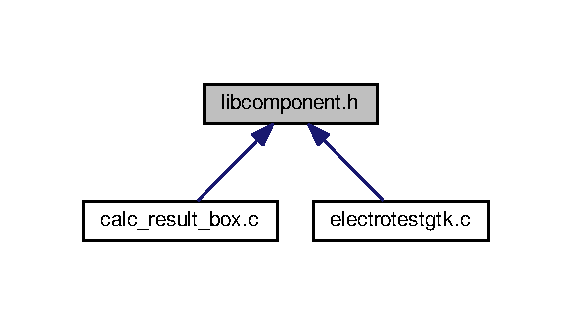
\includegraphics[width=275pt]{libcomponent_8h__dep__incl}
\end{center}
\end{figure}
\subsection*{Functions}
\begin{DoxyCompactItemize}
\item 
int \hyperlink{libcomponent_8h_ae430da75e2bfa147a1da4942b2684bd7}{findresistors} (float orig\+\_\+resistance, float $\ast$res\+\_\+array)
\end{DoxyCompactItemize}


\subsection{Function Documentation}
\index{libcomponent.\+h@{libcomponent.\+h}!findresistors@{findresistors}}
\index{findresistors@{findresistors}!libcomponent.\+h@{libcomponent.\+h}}
\subsubsection[{\texorpdfstring{findresistors(float orig\+\_\+resistance, float $\ast$res\+\_\+array)}{findresistors(float orig_resistance, float *res_array)}}]{\setlength{\rightskip}{0pt plus 5cm}int findresistors (
\begin{DoxyParamCaption}
\item[{float}]{orig\+\_\+resistance, }
\item[{float $\ast$}]{res\+\_\+array}
\end{DoxyParamCaption}
)}\hypertarget{libcomponent_8h_ae430da75e2bfa147a1da4942b2684bd7}{}\label{libcomponent_8h_ae430da75e2bfa147a1da4942b2684bd7}

\hypertarget{libpower_8h}{}\section{libpower.\+h File Reference}
\label{libpower_8h}\index{libpower.\+h@{libpower.\+h}}
{\ttfamily \#include $<$stdio.\+h$>$}\\*
{\ttfamily \#include $<$stdlib.\+h$>$}\\*
Include dependency graph for libpower.\+h\+:
\nopagebreak
\begin{figure}[H]
\begin{center}
\leavevmode
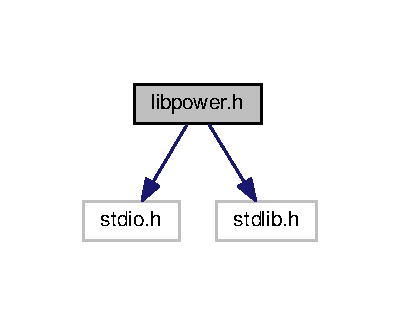
\includegraphics[width=192pt]{libpower_8h__incl}
\end{center}
\end{figure}
This graph shows which files directly or indirectly include this file\+:
\nopagebreak
\begin{figure}[H]
\begin{center}
\leavevmode
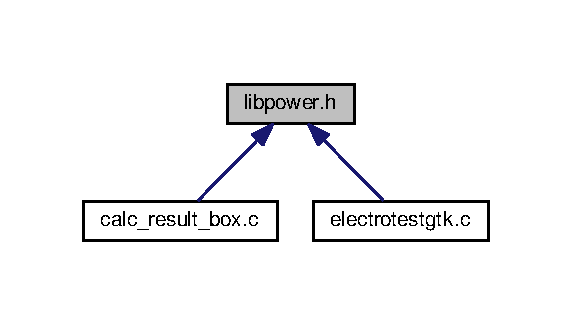
\includegraphics[width=275pt]{libpower_8h__dep__incl}
\end{center}
\end{figure}
\subsection*{Functions}
\begin{DoxyCompactItemize}
\item 
float \hyperlink{libpower_8h_ac075500b29b883b6c3ec6d6d6b91d73c}{calc\+\_\+power\+\_\+r} (float volt, float resistance)
\item 
float \hyperlink{libpower_8h_a1f0fd46c93dd4e37cd60b06026ba174f}{calc\+\_\+power\+\_\+i} (float volt, float current)
\end{DoxyCompactItemize}


\subsection{Function Documentation}
\index{libpower.\+h@{libpower.\+h}!calc\+\_\+power\+\_\+i@{calc\+\_\+power\+\_\+i}}
\index{calc\+\_\+power\+\_\+i@{calc\+\_\+power\+\_\+i}!libpower.\+h@{libpower.\+h}}
\subsubsection[{\texorpdfstring{calc\+\_\+power\+\_\+i(float volt, float current)}{calc_power_i(float volt, float current)}}]{\setlength{\rightskip}{0pt plus 5cm}float calc\+\_\+power\+\_\+i (
\begin{DoxyParamCaption}
\item[{float}]{volt, }
\item[{float}]{current}
\end{DoxyParamCaption}
)}\hypertarget{libpower_8h_a1f0fd46c93dd4e37cd60b06026ba174f}{}\label{libpower_8h_a1f0fd46c93dd4e37cd60b06026ba174f}
\index{libpower.\+h@{libpower.\+h}!calc\+\_\+power\+\_\+r@{calc\+\_\+power\+\_\+r}}
\index{calc\+\_\+power\+\_\+r@{calc\+\_\+power\+\_\+r}!libpower.\+h@{libpower.\+h}}
\subsubsection[{\texorpdfstring{calc\+\_\+power\+\_\+r(float volt, float resistance)}{calc_power_r(float volt, float resistance)}}]{\setlength{\rightskip}{0pt plus 5cm}float calc\+\_\+power\+\_\+r (
\begin{DoxyParamCaption}
\item[{float}]{volt, }
\item[{float}]{resistance}
\end{DoxyParamCaption}
)}\hypertarget{libpower_8h_ac075500b29b883b6c3ec6d6d6b91d73c}{}\label{libpower_8h_ac075500b29b883b6c3ec6d6d6b91d73c}

\hypertarget{libresistance_8h}{}\section{libresistance.\+h File Reference}
\label{libresistance_8h}\index{libresistance.\+h@{libresistance.\+h}}
This graph shows which files directly or indirectly include this file\+:
\nopagebreak
\begin{figure}[H]
\begin{center}
\leavevmode
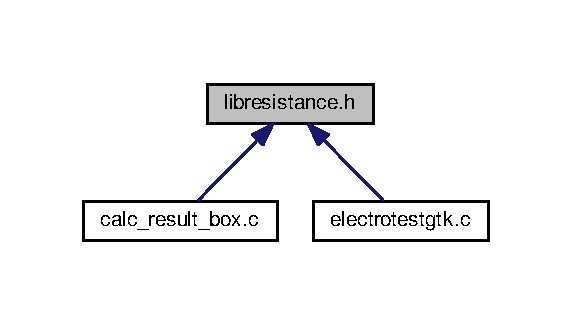
\includegraphics[width=275pt]{libresistance_8h__dep__incl}
\end{center}
\end{figure}
\subsection*{Functions}
\begin{DoxyCompactItemize}
\item 
float \hyperlink{libresistance_8h_a339b5f0f336eb492e36f9d6467678440}{calc\+\_\+resistance} (int count, char conn, float $\ast$array)
\end{DoxyCompactItemize}


\subsection{Function Documentation}
\index{libresistance.\+h@{libresistance.\+h}!calc\+\_\+resistance@{calc\+\_\+resistance}}
\index{calc\+\_\+resistance@{calc\+\_\+resistance}!libresistance.\+h@{libresistance.\+h}}
\subsubsection[{\texorpdfstring{calc\+\_\+resistance(int count, char conn, float $\ast$array)}{calc_resistance(int count, char conn, float *array)}}]{\setlength{\rightskip}{0pt plus 5cm}float calc\+\_\+resistance (
\begin{DoxyParamCaption}
\item[{int}]{count, }
\item[{char}]{conn, }
\item[{float $\ast$}]{array}
\end{DoxyParamCaption}
)}\hypertarget{libresistance_8h_a339b5f0f336eb492e36f9d6467678440}{}\label{libresistance_8h_a339b5f0f336eb492e36f9d6467678440}

\hypertarget{resistor__box_8c}{}\section{resistor\+\_\+box.\+c File Reference}
\label{resistor__box_8c}\index{resistor\+\_\+box.\+c@{resistor\+\_\+box.\+c}}
{\ttfamily \#include $<$gtk/gtk.\+h$>$}\\*
{\ttfamily \#include $<$stdlib.\+h$>$}\\*
{\ttfamily \#include \char`\"{}helper\+\_\+functions.\+h\char`\"{}}\\*
{\ttfamily \#include \char`\"{}resistor\+\_\+box.\+h\char`\"{}}\\*
Include dependency graph for resistor\+\_\+box.\+c\+:
\nopagebreak
\begin{figure}[H]
\begin{center}
\leavevmode
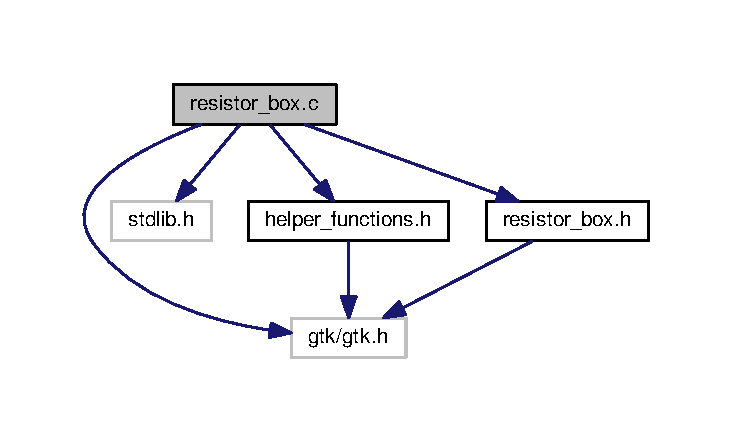
\includegraphics[width=350pt]{resistor__box_8c__incl}
\end{center}
\end{figure}
\subsection*{Functions}
\begin{DoxyCompactItemize}
\item 
Gtk\+Widget $\ast$ \hyperlink{resistor__box_8c_a85504126ef3346200383c77941978fa0}{resistor\+\_\+box\+\_\+new} (void)
\begin{DoxyCompactList}\small\item\em Constructor for resistor\+\_\+box G\+UI part. \end{DoxyCompactList}\item 
gfloat $\ast$ \hyperlink{resistor__box_8c_a4b211b67cb036e4975150e165c5bf360}{update\+\_\+resistor\+\_\+values} (Gtk\+Widget $\ast$resistor\+\_\+box, gfloat $\ast$value\+\_\+array)
\begin{DoxyCompactList}\small\item\em Updates the value\+\_\+array with values from the G\+UI. \end{DoxyCompactList}\end{DoxyCompactItemize}
\subsection*{Variables}
\begin{DoxyCompactItemize}
\item 
char $\ast$const \hyperlink{resistor__box_8c_ac7511da732d0573c995c8a23b327ca50}{resistor\+\_\+names} \mbox{[}$\,$\mbox{]} = \{ \char`\"{}res1\char`\"{}, \char`\"{}res2\char`\"{}, \char`\"{}res3\char`\"{} \}
\item 
char $\ast$const \hyperlink{resistor__box_8c_a51c65d2cdfcb1fb2352797184d054e06}{resistor\+\_\+labels} \mbox{[}$\,$\mbox{]} = \{\char`\"{}1\+:\char`\"{}, \char`\"{}2\+:\char`\"{}, \char`\"{}3\+:\char`\"{}\}
\end{DoxyCompactItemize}


\subsection{Function Documentation}
\index{resistor\+\_\+box.\+c@{resistor\+\_\+box.\+c}!resistor\+\_\+box\+\_\+new@{resistor\+\_\+box\+\_\+new}}
\index{resistor\+\_\+box\+\_\+new@{resistor\+\_\+box\+\_\+new}!resistor\+\_\+box.\+c@{resistor\+\_\+box.\+c}}
\subsubsection[{\texorpdfstring{resistor\+\_\+box\+\_\+new(void)}{resistor_box_new(void)}}]{\setlength{\rightskip}{0pt plus 5cm}Gtk\+Widget$\ast$ resistor\+\_\+box\+\_\+new (
\begin{DoxyParamCaption}
\item[{void}]{}
\end{DoxyParamCaption}
)}\hypertarget{resistor__box_8c_a85504126ef3346200383c77941978fa0}{}\label{resistor__box_8c_a85504126ef3346200383c77941978fa0}


Constructor for resistor\+\_\+box G\+UI part. 

This G\+UI part contains three resistor input field.

\begin{DoxyReturn}{Returns}
Gtk\+Widget Contains the constructed G\+UI part. 
\end{DoxyReturn}
\index{resistor\+\_\+box.\+c@{resistor\+\_\+box.\+c}!update\+\_\+resistor\+\_\+values@{update\+\_\+resistor\+\_\+values}}
\index{update\+\_\+resistor\+\_\+values@{update\+\_\+resistor\+\_\+values}!resistor\+\_\+box.\+c@{resistor\+\_\+box.\+c}}
\subsubsection[{\texorpdfstring{update\+\_\+resistor\+\_\+values(\+Gtk\+Widget $\ast$resistor\+\_\+box, gfloat $\ast$value\+\_\+array)}{update_resistor_values(GtkWidget *resistor_box, gfloat *value_array)}}]{\setlength{\rightskip}{0pt plus 5cm}gfloat$\ast$ update\+\_\+resistor\+\_\+values (
\begin{DoxyParamCaption}
\item[{Gtk\+Widget $\ast$}]{resistor\+\_\+box, }
\item[{gfloat $\ast$}]{value\+\_\+array}
\end{DoxyParamCaption}
)}\hypertarget{resistor__box_8c_a4b211b67cb036e4975150e165c5bf360}{}\label{resistor__box_8c_a4b211b67cb036e4975150e165c5bf360}


Updates the value\+\_\+array with values from the G\+UI. 

The Function assumes a gfloat array of size 3.


\begin{DoxyParams}{Parameters}
{\em resistor\+\_\+box} & The G\+UI part to access the user input.  Float array of size 3 that contains the resistor values \\
\hline
\end{DoxyParams}


\subsection{Variable Documentation}
\index{resistor\+\_\+box.\+c@{resistor\+\_\+box.\+c}!resistor\+\_\+labels@{resistor\+\_\+labels}}
\index{resistor\+\_\+labels@{resistor\+\_\+labels}!resistor\+\_\+box.\+c@{resistor\+\_\+box.\+c}}
\subsubsection[{\texorpdfstring{resistor\+\_\+labels}{resistor_labels}}]{\setlength{\rightskip}{0pt plus 5cm}char$\ast$ const resistor\+\_\+labels\mbox{[}$\,$\mbox{]} = \{\char`\"{}1\+:\char`\"{}, \char`\"{}2\+:\char`\"{}, \char`\"{}3\+:\char`\"{}\}}\hypertarget{resistor__box_8c_a51c65d2cdfcb1fb2352797184d054e06}{}\label{resistor__box_8c_a51c65d2cdfcb1fb2352797184d054e06}
\index{resistor\+\_\+box.\+c@{resistor\+\_\+box.\+c}!resistor\+\_\+names@{resistor\+\_\+names}}
\index{resistor\+\_\+names@{resistor\+\_\+names}!resistor\+\_\+box.\+c@{resistor\+\_\+box.\+c}}
\subsubsection[{\texorpdfstring{resistor\+\_\+names}{resistor_names}}]{\setlength{\rightskip}{0pt plus 5cm}char$\ast$ const resistor\+\_\+names\mbox{[}$\,$\mbox{]} = \{ \char`\"{}res1\char`\"{}, \char`\"{}res2\char`\"{}, \char`\"{}res3\char`\"{} \}}\hypertarget{resistor__box_8c_ac7511da732d0573c995c8a23b327ca50}{}\label{resistor__box_8c_ac7511da732d0573c995c8a23b327ca50}

\hypertarget{resistor__box_8h}{}\section{resistor\+\_\+box.\+h File Reference}
\label{resistor__box_8h}\index{resistor\+\_\+box.\+h@{resistor\+\_\+box.\+h}}
{\ttfamily \#include $<$gtk/gtk.\+h$>$}\\*
Include dependency graph for resistor\+\_\+box.\+h\+:
\nopagebreak
\begin{figure}[H]
\begin{center}
\leavevmode
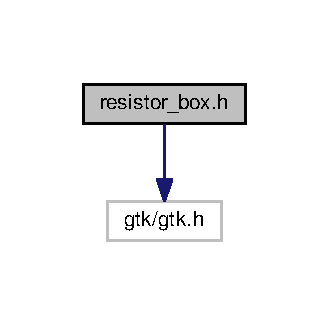
\includegraphics[width=158pt]{resistor__box_8h__incl}
\end{center}
\end{figure}
This graph shows which files directly or indirectly include this file\+:
\nopagebreak
\begin{figure}[H]
\begin{center}
\leavevmode
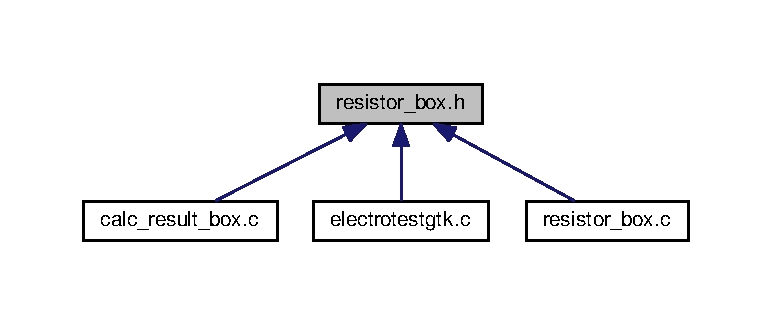
\includegraphics[width=350pt]{resistor__box_8h__dep__incl}
\end{center}
\end{figure}
\subsection*{Functions}
\begin{DoxyCompactItemize}
\item 
Gtk\+Widget $\ast$ \hyperlink{resistor__box_8h_a85504126ef3346200383c77941978fa0}{resistor\+\_\+box\+\_\+new} (void)
\begin{DoxyCompactList}\small\item\em Constructor for resistor\+\_\+box G\+UI part. \end{DoxyCompactList}\item 
float $\ast$ \hyperlink{resistor__box_8h_a29bd18149b7899115aa462ec941e1bc2}{update\+\_\+resistor\+\_\+values} (Gtk\+Widget $\ast$resistor\+\_\+box, float $\ast$value\+\_\+array)
\begin{DoxyCompactList}\small\item\em Updates the value\+\_\+array with values from the G\+UI. \end{DoxyCompactList}\end{DoxyCompactItemize}


\subsection{Function Documentation}
\index{resistor\+\_\+box.\+h@{resistor\+\_\+box.\+h}!resistor\+\_\+box\+\_\+new@{resistor\+\_\+box\+\_\+new}}
\index{resistor\+\_\+box\+\_\+new@{resistor\+\_\+box\+\_\+new}!resistor\+\_\+box.\+h@{resistor\+\_\+box.\+h}}
\subsubsection[{\texorpdfstring{resistor\+\_\+box\+\_\+new(void)}{resistor_box_new(void)}}]{\setlength{\rightskip}{0pt plus 5cm}Gtk\+Widget$\ast$ resistor\+\_\+box\+\_\+new (
\begin{DoxyParamCaption}
\item[{void}]{}
\end{DoxyParamCaption}
)}\hypertarget{resistor__box_8h_a85504126ef3346200383c77941978fa0}{}\label{resistor__box_8h_a85504126ef3346200383c77941978fa0}


Constructor for resistor\+\_\+box G\+UI part. 

This G\+UI part contains three resistor input field.

\begin{DoxyReturn}{Returns}
Gtk\+Widget Contains the constructed G\+UI part. 
\end{DoxyReturn}
\index{resistor\+\_\+box.\+h@{resistor\+\_\+box.\+h}!update\+\_\+resistor\+\_\+values@{update\+\_\+resistor\+\_\+values}}
\index{update\+\_\+resistor\+\_\+values@{update\+\_\+resistor\+\_\+values}!resistor\+\_\+box.\+h@{resistor\+\_\+box.\+h}}
\subsubsection[{\texorpdfstring{update\+\_\+resistor\+\_\+values(\+Gtk\+Widget $\ast$resistor\+\_\+box, float $\ast$value\+\_\+array)}{update_resistor_values(GtkWidget *resistor_box, float *value_array)}}]{\setlength{\rightskip}{0pt plus 5cm}float$\ast$ update\+\_\+resistor\+\_\+values (
\begin{DoxyParamCaption}
\item[{Gtk\+Widget $\ast$}]{resistor\+\_\+box, }
\item[{float $\ast$}]{value\+\_\+array}
\end{DoxyParamCaption}
)}\hypertarget{resistor__box_8h_a29bd18149b7899115aa462ec941e1bc2}{}\label{resistor__box_8h_a29bd18149b7899115aa462ec941e1bc2}


Updates the value\+\_\+array with values from the G\+UI. 

The Function assumes a gfloat array of size 3.


\begin{DoxyParams}{Parameters}
{\em resistor\+\_\+box} & The G\+UI part to access the user input.  Float array of size 3 that contains the resistor values \\
\hline
\end{DoxyParams}

\hypertarget{voltage__box_8c}{}\section{voltage\+\_\+box.\+c File Reference}
\label{voltage__box_8c}\index{voltage\+\_\+box.\+c@{voltage\+\_\+box.\+c}}
{\ttfamily \#include $<$stdlib.\+h$>$}\\*
{\ttfamily \#include \char`\"{}voltage\+\_\+box.\+h\char`\"{}}\\*
{\ttfamily \#include \char`\"{}helper\+\_\+functions.\+h\char`\"{}}\\*
Include dependency graph for voltage\+\_\+box.\+c\+:
\nopagebreak
\begin{figure}[H]
\begin{center}
\leavevmode
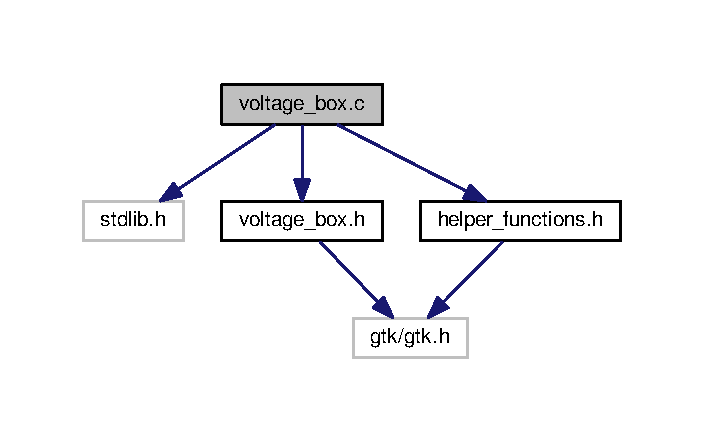
\includegraphics[width=338pt]{voltage__box_8c__incl}
\end{center}
\end{figure}
\subsection*{Functions}
\begin{DoxyCompactItemize}
\item 
Gtk\+Widget $\ast$ \hyperlink{voltage__box_8c_a5e1085883b0c48140cba70c17a46ae97}{voltage\+\_\+box\+\_\+new} (void)
\begin{DoxyCompactList}\small\item\em Constructor for voltage\+\_\+box G\+UI element. \end{DoxyCompactList}\item 
float \hyperlink{voltage__box_8c_a02e5dac060c6b706fd50fb4fcd27f9a2}{get\+\_\+voltage} (Gtk\+Widget $\ast$voltage\+\_\+box)
\begin{DoxyCompactList}\small\item\em Retrieve voltage value from G\+UI entry field. \end{DoxyCompactList}\end{DoxyCompactItemize}


\subsection{Function Documentation}
\index{voltage\+\_\+box.\+c@{voltage\+\_\+box.\+c}!get\+\_\+voltage@{get\+\_\+voltage}}
\index{get\+\_\+voltage@{get\+\_\+voltage}!voltage\+\_\+box.\+c@{voltage\+\_\+box.\+c}}
\subsubsection[{\texorpdfstring{get\+\_\+voltage(\+Gtk\+Widget $\ast$voltage\+\_\+box)}{get_voltage(GtkWidget *voltage_box)}}]{\setlength{\rightskip}{0pt plus 5cm}float get\+\_\+voltage (
\begin{DoxyParamCaption}
\item[{Gtk\+Widget $\ast$}]{voltage\+\_\+box}
\end{DoxyParamCaption}
)}\hypertarget{voltage__box_8c_a02e5dac060c6b706fd50fb4fcd27f9a2}{}\label{voltage__box_8c_a02e5dac060c6b706fd50fb4fcd27f9a2}


Retrieve voltage value from G\+UI entry field. 

Retrieves float value of the voltage input box. The function needs a reference/pointer to the G\+UI element.


\begin{DoxyParams}{Parameters}
{\em voltage\+\_\+box} & Gtk\+Widget G\+UI element voltage\+\_\+box \\
\hline
\end{DoxyParams}
\begin{DoxyReturn}{Returns}
float value of the current set voltage value in the G\+UI 
\end{DoxyReturn}
\index{voltage\+\_\+box.\+c@{voltage\+\_\+box.\+c}!voltage\+\_\+box\+\_\+new@{voltage\+\_\+box\+\_\+new}}
\index{voltage\+\_\+box\+\_\+new@{voltage\+\_\+box\+\_\+new}!voltage\+\_\+box.\+c@{voltage\+\_\+box.\+c}}
\subsubsection[{\texorpdfstring{voltage\+\_\+box\+\_\+new(void)}{voltage_box_new(void)}}]{\setlength{\rightskip}{0pt plus 5cm}Gtk\+Widget$\ast$ voltage\+\_\+box\+\_\+new (
\begin{DoxyParamCaption}
\item[{void}]{}
\end{DoxyParamCaption}
)}\hypertarget{voltage__box_8c_a5e1085883b0c48140cba70c17a46ae97}{}\label{voltage__box_8c_a5e1085883b0c48140cba70c17a46ae97}


Constructor for voltage\+\_\+box G\+UI element. 

Constructs the voltage\+\_\+box G\+UI element which contains the entry field for setting the voltage.

\begin{DoxyReturn}{Returns}
Gtk\+Widget A voltage\+\_\+box G\+UI Element 
\end{DoxyReturn}

\hypertarget{voltage__box_8h}{}\section{voltage\+\_\+box.\+h File Reference}
\label{voltage__box_8h}\index{voltage\+\_\+box.\+h@{voltage\+\_\+box.\+h}}
{\ttfamily \#include $<$gtk/gtk.\+h$>$}\\*
Include dependency graph for voltage\+\_\+box.\+h\+:
\nopagebreak
\begin{figure}[H]
\begin{center}
\leavevmode
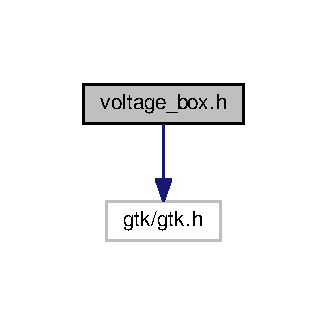
\includegraphics[width=157pt]{voltage__box_8h__incl}
\end{center}
\end{figure}
This graph shows which files directly or indirectly include this file\+:
\nopagebreak
\begin{figure}[H]
\begin{center}
\leavevmode
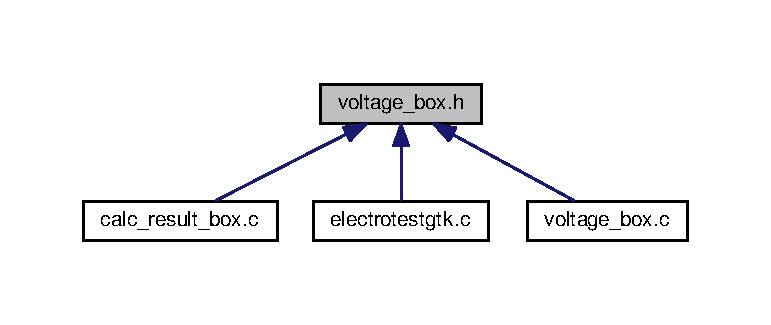
\includegraphics[width=350pt]{voltage__box_8h__dep__incl}
\end{center}
\end{figure}
\subsection*{Functions}
\begin{DoxyCompactItemize}
\item 
Gtk\+Widget $\ast$ \hyperlink{voltage__box_8h_a5e1085883b0c48140cba70c17a46ae97}{voltage\+\_\+box\+\_\+new} (void)
\begin{DoxyCompactList}\small\item\em Constructor for voltage\+\_\+box G\+UI element. \end{DoxyCompactList}\item 
float \hyperlink{voltage__box_8h_a02e5dac060c6b706fd50fb4fcd27f9a2}{get\+\_\+voltage} (Gtk\+Widget $\ast$voltage\+\_\+box)
\begin{DoxyCompactList}\small\item\em Retrieve voltage value from G\+UI entry field. \end{DoxyCompactList}\end{DoxyCompactItemize}


\subsection{Function Documentation}
\index{voltage\+\_\+box.\+h@{voltage\+\_\+box.\+h}!get\+\_\+voltage@{get\+\_\+voltage}}
\index{get\+\_\+voltage@{get\+\_\+voltage}!voltage\+\_\+box.\+h@{voltage\+\_\+box.\+h}}
\subsubsection[{\texorpdfstring{get\+\_\+voltage(\+Gtk\+Widget $\ast$voltage\+\_\+box)}{get_voltage(GtkWidget *voltage_box)}}]{\setlength{\rightskip}{0pt plus 5cm}float get\+\_\+voltage (
\begin{DoxyParamCaption}
\item[{Gtk\+Widget $\ast$}]{voltage\+\_\+box}
\end{DoxyParamCaption}
)}\hypertarget{voltage__box_8h_a02e5dac060c6b706fd50fb4fcd27f9a2}{}\label{voltage__box_8h_a02e5dac060c6b706fd50fb4fcd27f9a2}


Retrieve voltage value from G\+UI entry field. 

Retrieves float value of the voltage input box. The function needs a reference/pointer to the G\+UI element.


\begin{DoxyParams}{Parameters}
{\em voltage\+\_\+box} & Gtk\+Widget G\+UI element voltage\+\_\+box \\
\hline
\end{DoxyParams}
\begin{DoxyReturn}{Returns}
float value of the current set voltage value in the G\+UI 
\end{DoxyReturn}
\index{voltage\+\_\+box.\+h@{voltage\+\_\+box.\+h}!voltage\+\_\+box\+\_\+new@{voltage\+\_\+box\+\_\+new}}
\index{voltage\+\_\+box\+\_\+new@{voltage\+\_\+box\+\_\+new}!voltage\+\_\+box.\+h@{voltage\+\_\+box.\+h}}
\subsubsection[{\texorpdfstring{voltage\+\_\+box\+\_\+new(void)}{voltage_box_new(void)}}]{\setlength{\rightskip}{0pt plus 5cm}Gtk\+Widget$\ast$ voltage\+\_\+box\+\_\+new (
\begin{DoxyParamCaption}
\item[{void}]{}
\end{DoxyParamCaption}
)}\hypertarget{voltage__box_8h_a5e1085883b0c48140cba70c17a46ae97}{}\label{voltage__box_8h_a5e1085883b0c48140cba70c17a46ae97}


Constructor for voltage\+\_\+box G\+UI element. 

Constructs the voltage\+\_\+box G\+UI element which contains the entry field for setting the voltage.

\begin{DoxyReturn}{Returns}
Gtk\+Widget A voltage\+\_\+box G\+UI Element 
\end{DoxyReturn}

%--- End generated contents ---

% Index
\backmatter
\newpage
\phantomsection
\clearemptydoublepage
\addcontentsline{toc}{chapter}{Index}
\printindex

\end{document}
